%\subsection{An\'alisis suplementarios}\label{sec:escenario1_supl}
\par Teniendo una gran cantidad de informaci\'on capturada en las distintas redes
que componen este escenario, corresponde quiz\'as hacer un an\'alisis un poco
m\'as profundo sobre las distintas variables que podemos identificar y guardar
durante la etapa de \textit{sniffing}.

\par Estas variables pueden ser muchas. En particular identificamos dos variables,
por ah\'i un tanto inmediatas y no muy complejas, pero no por ello menos importantes
o menos propensas a otorgarnos informaci\'on. Estamos hablando de la parametrizaci\'on
seg\'un el tiempo (cuando fue capturada cierta informaci\'on) y la cantidad (cuanta
informaci\'on).

\par As\'i pues, en un principio resulta interesante para comprender el comportamiento
de las redes ver el vol\'umen de paquetes ARP durante per\'iodos m\'as cortos. Hasta
este momento, en este escenario nos estuvimos concentrando en comprender a toda la
informaci\'on capturada como 2 grandes fuentes de informaci\'on (fuente origen y
fuente destino). Proponemos, entonces, observar que ocurre m\'as granularmente
al comprender a las fuentes de informaci\'on no como un \textit{todo}, sino analizando
que ocurr\'io cada d\'ia de captura.


\subsubsection{Vol\'umen de paquetes ARP por d\'ia/hora}
\par En la figura \ref{fig:arp_por_hora} se pueden observar como
va evolucionando la cantidad de paquetes capturados en per\'iodos de 60 minutos, y a
su vez comparar este comportamiento en los diferentes d\'ias.

\begin{figure*}[!b]
    \begin{tabular}{cc}
        \centering
        \subfloat[\nameref{itm:vlan10}]{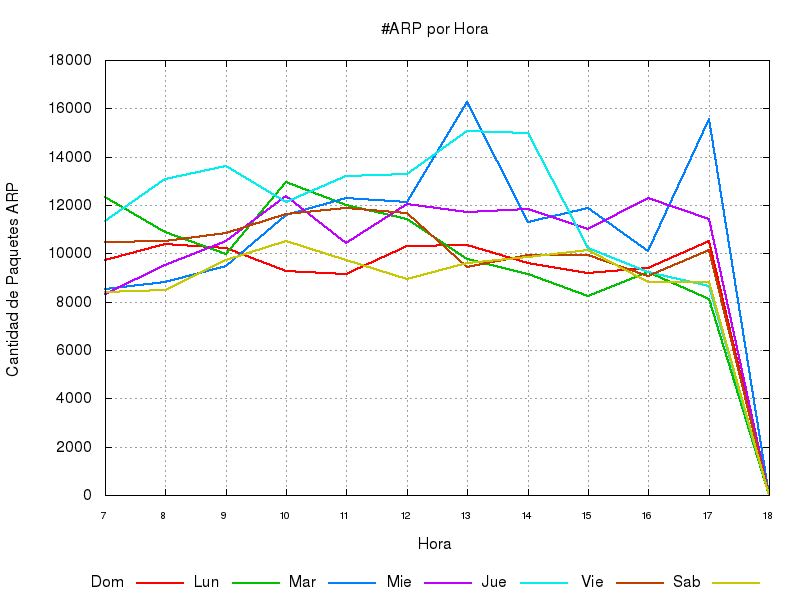
\includegraphics[width=0.5\textwidth]{img/graph/escenario_1/vlan10/vlan10_arp_per_hour_lines}} &
        \subfloat[\nameref{itm:vlan20}]{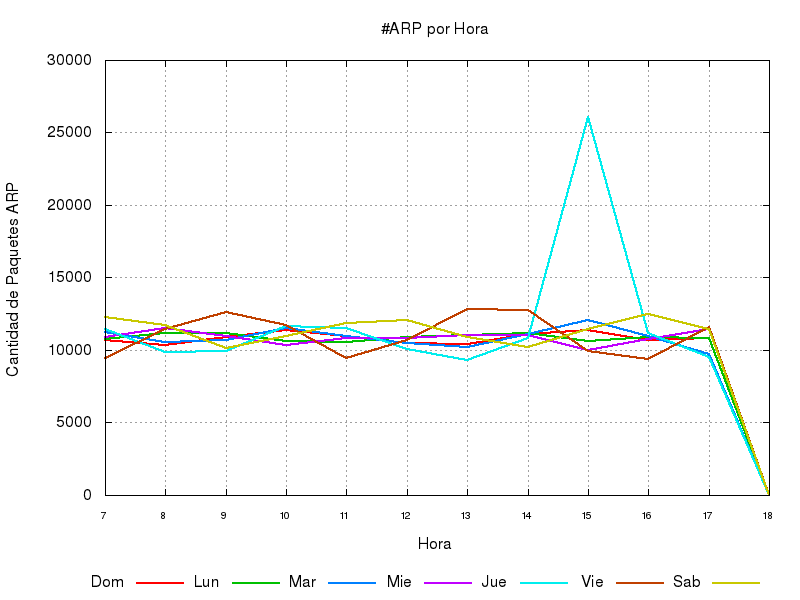
\includegraphics[width=0.5\textwidth]{img/graph/escenario_1/vlan20/vlan20_arp_per_hour_lines}} \\
        \subfloat[\nameref{itm:vlan40}]{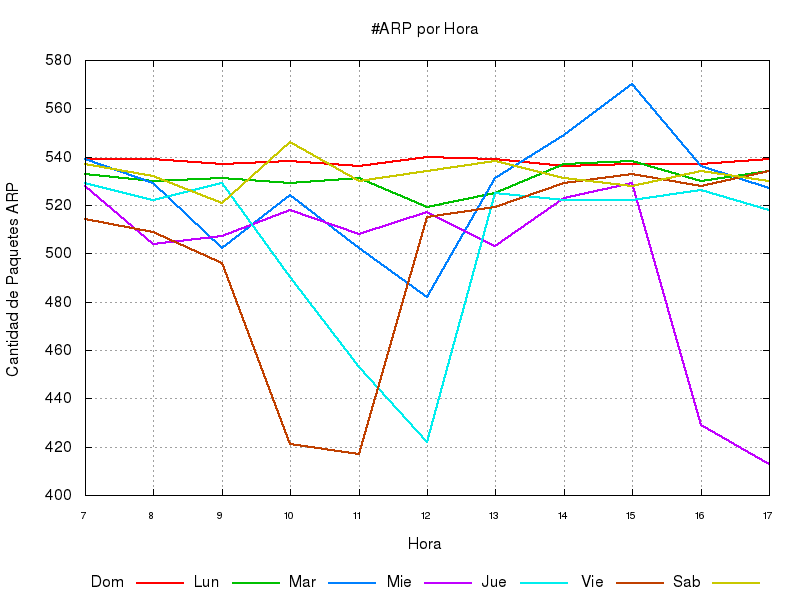
\includegraphics[width=0.5\textwidth]{img/graph/escenario_1/vlan40/vlan40_arp_per_hour_lines}} &
        \subfloat[\nameref{itm:vlan1}]{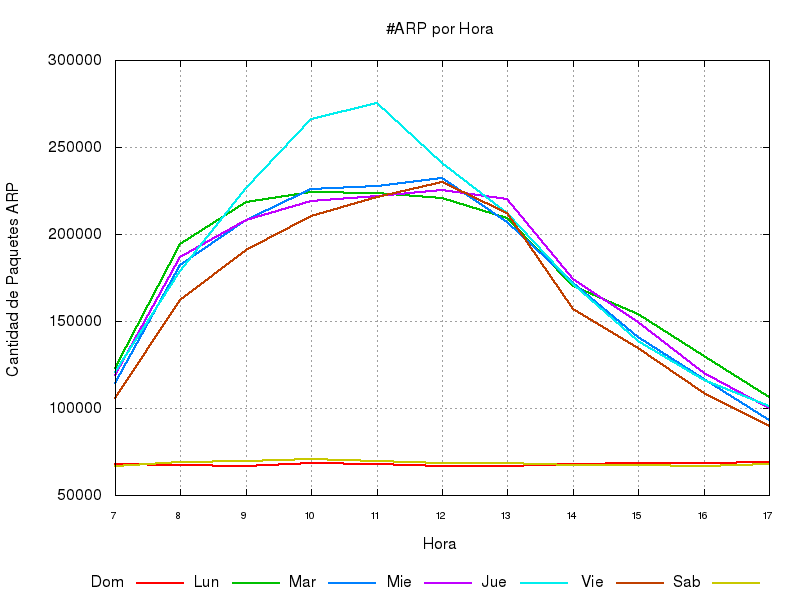
\includegraphics[width=0.5\textwidth]{img/graph/escenario_1/vlan1/vlan1_arp_per_hour_lines}} \\
    \end{tabular}
    \caption{Cantidad de paquetes ARP por hora}
    \label{fig:arp_por_hora}
\end{figure*}

\par Como primer resultado, que claramente salta a primera vista, es que el
comportamiento\footnote{Siempre pensado respecto de los paquetes ARP que se
encuentran en la red.} de las redes es bastante ca\'otico en cuanto a la cantidad
de paquetes por hora y d\'ia.

\par Claramente, el experimento realizado no nos permite decir exactamente que
est\'a ocurriendo en la red, pero si vemos que en el aspecto de como var\'ia
el vol\'umen de estos paquetes (y por lo tanto, una parte importante de la
congesti\'on de la LAN) nos encontramos con tres casos que parec\'ieran
seguir patron, mientras que la red de \nameref{itm:vlan40} pareciese,
\textit{a priori}, no hacerlo

\par Respecto de esto, y con el conocimiento que se tiene de que dispositivos/%
usuarios participan de la red, queda claro que el comportamiento aleatorio de
los usuarios con sus terminales (e incluso con terminales que un d\'ia est\'an
y otro no; o incluso que se conectan a la red en franjas horarias dispares)
tiene un impacto direct en la cantidad de paquetes que circulan en la red. M\'as
interesante, se puede observar que el vol\'umen es claramente m\'as alto en los
alrededores del mediod\'ia (comparando cada d\'ia en su variaci\'on por hora) y
en los d\'ias intermedios de la semana (comparando una misma hora pero en distintos
d\'ias)

\par Este \'ultimo detalle no s\'olo ocurre en la red de \nameref{itm:vlan10},
sino que tambi\'en se puede observar, y mucho m\'as marcado, en la red
\nameref{itm:vlan1}. Se observa aqu\'i que el vol\'umen es muy estable, bajo y
parejo los S\'abados y Domingos, y que durante los d\'ias de la semana se observa
un vol\'umen m\'as grande en la franja horaria de 9 a 14 hs, que luego se reduce
considerablemente hacia el fin de la jornada laboral\footnote{En particular, la
mayor\'ia de los usuarios de las redes observadas utiliza la red entre las 7 y
las 15 hs}. 

\par A pesar de ver este comportamiento similar, debemos aclarar
que los vol\'umenes de ambas redes son claramente distintos. Sin ir m\'as lejos,
en el caso promedio, la red \nameref{itm:vlan1} tiene 20 veces m\'as paquetes ARP
que \nameref{itm:vlan10}. Es decir, podr\'iamos tener una variacia\'on m\'as
grande, nominalmente hablando, dentro de esta red. Pero tomando en cuenta
el vol\'umen total y la cantidad de paquetes, es admitible la comparaci\'on.

\par Algo remarcable de esta similitud reci\'en expuesta, es que la red de
\nameref{itm:vlan1} tiene muchos servidores aparte de usuarios, y si obsevamos
el grafico correspondiente a la red \nameref{itm:vlan20}, veremos un vol\'umen
similar al de la red \nameref{itm:vlan10} y de comportamiento igualmente
dispar\footnote{M\'as all\'a del \textit{outlier} correspondiente a las
15 hs del Jueves. Probablemente hubo alguna instalaci\'on de servidores o
software en los mismos que impactaron en la red.}. Al observar
una red que combina, esperablemente, los comportamientos de estos dos tipos
de redes, nos encontramos con una red que tiene un vol\'umen base seguramente
dependiente de los servidores\footnote{ya que estos no suelen desconectarse y
tienen un comportamiento m\'as estable que las terminales de usuarios}
(claramente observable en las l\'ineas que corresponde nal S\'abado y Domingo)
y luego durante los d\'ias de semana con la afluencia de las terminales de
los empleados, se ve como el vol\'umen se incrementa not\'ablemente.

\par En cuanto a la red de \nameref{itm:vlan40}, simplemente podemos ver
que maneja un vol\'umen que no pareciese seguir un patr\'on respecto
de las horas ni los d\'ias. No s\'olo eso, sino que el vol\'umen que manejan
pareciera ser m\'as estable que en el resto de los casos (mucha menos
variaci\'on de vol\'umen por hora y d\'ia). As\'i pues, podemos determinar
que estos dispositivos (al menos los que se utilizan en esta red, no podr\'iamos
hacer la siguiente aserci\'on para todas las redes de telefon\'ia) hacen un
uso distinguiblemente menor en cuanto a la identificaci\'on de las \textit{MAC}
de los dem\'as. Esto tambi\'en podr\'ia deberse a que la cantidad de dispositivos
conectados es mucho menor y por ah\'i los dispositivos tienen suficiente
espacio en su tabla ARP para no requer\'i consultar a la red tan seguido por la
resoluci\'on de una IP.


\subsubsection{Relaci\'on entrop\'ia - vol\'umen diario de paquetes ARP}
\par Habiendo analizado el vol\'umen de los paquetes ARP en cada red
seg\'un la variable temporal, ahora nos interesa ver si la variabilidad
de este vol\'umen tiene alg\'una relaci\'on con la entrop\'ia. A su vez,
un dato interesante a observar es ver si la entrop\'ia mantiene un comportamiento
estable a lo largo del tiempo o si var\'ia mucho respecto de la informaci\'on
que se capturo en un determinado \textit{frame} de tiempo.

\par En la figura \ref{fig:arp_vs_entropia} podemos observar ambas cosas.
Por un lado se puede observar como var\'ia la entrop\'ia de cada fuente
a medida que pasan los d\'ias de las capturas, y a su vez, en un segundo
plano con un histograma, se observa como var\'ia el vol\'umen de paquetes
en esos d\'ias. Ambos datos graficados trabajan en una escala distinta, ya que las
magnitudes de la cantidad de par\'ametros y la entrop\'ia poco tienen 
que ver\footnote{Lo que nos interesa observar es como se relacionan los comportamientos,
no sus magnitudes.}.

\begin{figure*}[!ht]
    \begin{tabular}{cc}
        \centering
        \subfloat[\nameref{itm:vlan10}]{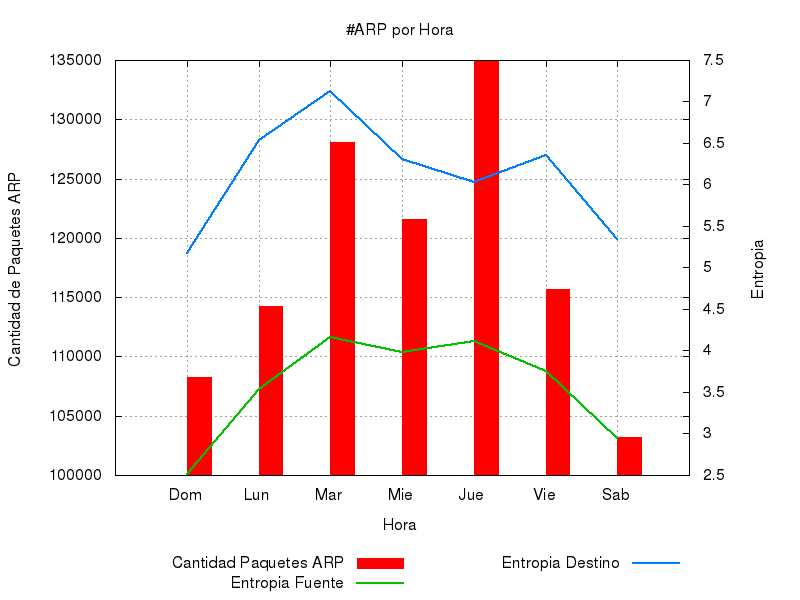
\includegraphics[width=0.5\textwidth]{img/graph/escenario_1/vlan10/vlan10_arp_vs_entropia}} &
        \subfloat[\nameref{itm:vlan20}]{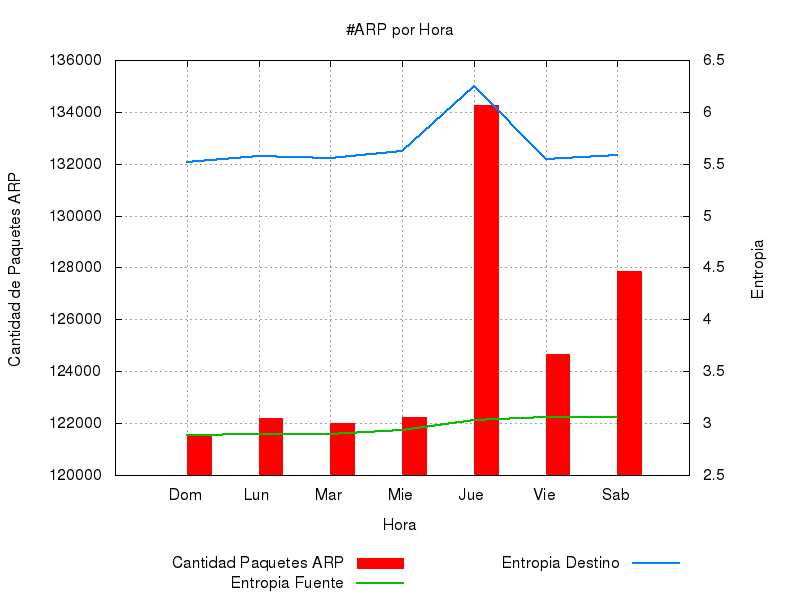
\includegraphics[width=0.5\textwidth]{img/graph/escenario_1/vlan20/vlan20_arp_vs_entropia}} \\
        \subfloat[\nameref{itm:vlan40}]{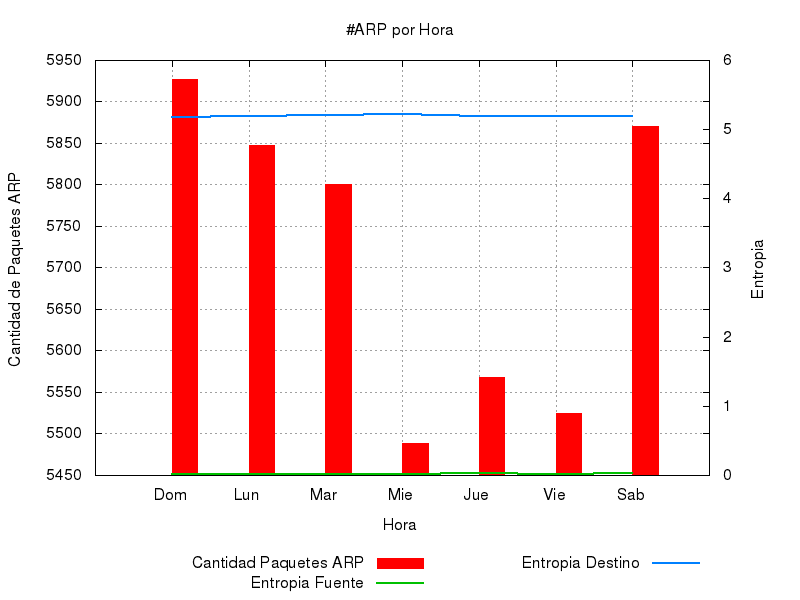
\includegraphics[width=0.5\textwidth]{img/graph/escenario_1/vlan40/vlan40_arp_vs_entropia}} &
        \subfloat[\nameref{itm:vlan1}]{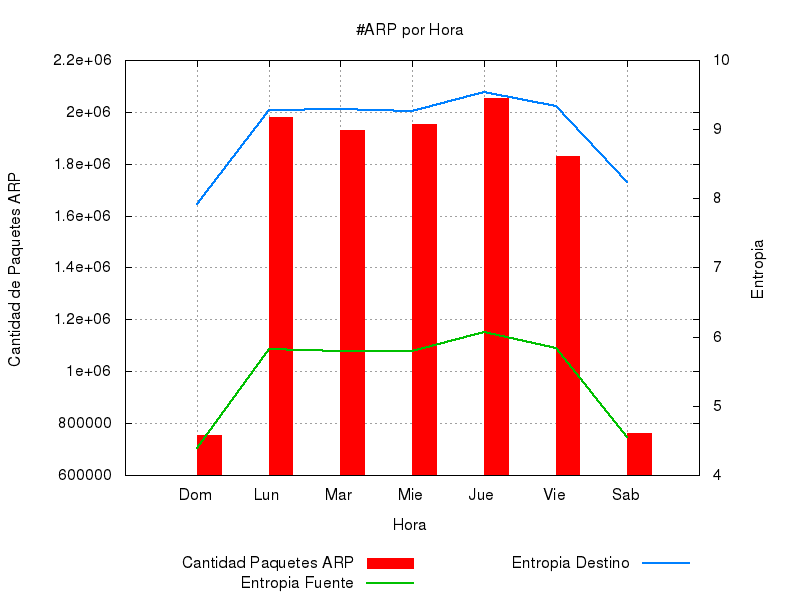
\includegraphics[width=0.5\textwidth]{img/graph/escenario_1/vlan1/vlan1_arp_vs_entropia}} \\
    \end{tabular}
    \caption{Cantidad de paquetes ARP por hora}
    \label{fig:arp_vs_entropia}
\end{figure*}

\par Se observa inicialmente que los comportamientos de la entrop\'ia de
la fuente de origen y destino pareciesen ser similares. Es decir, como
medida de informaci\'on/incertidumbre, vemos que dos fuentes de informaci\'on
que se observan a partir de los mismos paquetes (aunque sea en campos distintos)
demuestran que en cuanto a paquetes ARP, la variaci\'on del comportamiento
de la red afecta de forma muy parecida a ambas fuentes.

\par Por otro lado nos encontramos con que la entrop\'ia no var\'ia necesariamente
seg\'un var\'ia el vol\'umen de paquetes. De hecho, vemos que esto si ocurre
en todas las redes observadas salvo la de \nameref{itm:vlan40}. Pero este \'ultimo
caso nos da la pauta de que no se puede asumir este comportamiento como regla.

\par Analizando ahora los 3 casos donde la entrop\'ia efectivamente var\'ia
con el vol\'umen de paquetes, vemos tambi\'en que no parece haber una relaci\'on
fija entre las entrop\'ias de las dos fuentes. De hecho, se puede observar
que con el incremento del vol\'umen de paquetes, en la red de \nameref{itm:vlan1}
se ve que afecta de igual manera a la entrop\'ia de ambas fuentes\footnote{Por
abuso de notaci\'on decimos que se afecta a la entrop\'ia y no a la fuente en
si misma, ya que la entrop\'ia es un valor observacional de la fuente} mientras
que en \nameref{itm:vlan10} la entrop\'ia de la red de \nameref{itm:vlan10}
afecta a las entrop\'ias de forma inversa (una aumenta y la otra disminuye).

\par Ahora bien, viendo que aumentan los paquetes ARP en un determinado momento,
y viendo como var\'ian las entrop\'ias de la fuente, se puede llegar a alguna
que otra conclusi\'on interesante.

\par Por un lado, haciendo foco en la red de \nameref{itm:vlan20}, al observar
que la entrop\'ia de la fuente origen aumenta acorde aumenta la cantidad
de paquetes capturados durante el Jueves, podemos intuir que alguna(s)
de las terminales de la red est\'an siendo consultada mucho m\'as que en otros d\'ias,
ya que la incertidumbre\footnote{Otra forma de pensar a la entrop\'ia} a aumentado,
distribuyendo la probabilidad de aparici\'on de las IPs de forma m\'as equilibrada%
\footnote{Recordamos que la entrop\'ia es m\'axima para una fuente de informaci\'on
equiprobable.}.

\par En cambio, al observar la red \nameref{itm:vlan10}, observamos que ocurren
dos cosas:
\begin{enumerate*}[label=\itshape\alph*\upshape)]
    \item La entrop\'ia de la fuente destino disminuye notoriamente cuando el Jueves
    aumenta el vol\'umen de paquetes, d\'andonos la pauta de que este aumento fue
    destinado a una cantidad a\'un m\'as concentrada de IPs de lo que ven\'ia siendo; y

    \item La entrop\'ia de la fuente origen disminuye cuando llegamos al Viernes
    y se vuelve a tener un vol\'umen m\'as acorde al promedio de la fuente. En este
    caso, podemos imaginar que los paquetes que ya no aparecen m\'as en el dominio
    de colisi\'on eran env\'iados el d\'ia anterior muy probablemente desde un conjunto grande
    de IPs, ya que ahora al bajar el vol\'umen de paquetes vemos que la probabilidad
    se encuentra m\'as concentrada en un conjunto m\'as peque\~nos de IPs (pues la
    entrop\'ia disminuy\'o).
\end{enumerate*}

\par As\'i pues, si bien podemos concluir que la entrop\'ia no tiene un comportamiento
fijo respecto al vol\'umen de s\'imbolos capturados de la fuente informaci\'on, nos
puede da cierta direcci\'on en cuanto a que debe haber pasado acorde al cambi\'o del
vol\'umen. No es lo mismo que la entrop\'ia aumente o disminuya si la cantidad de
paquetes/mensajes capturados/enviados de la fuente, lo cual nos
ayuda a entender que puede estar ocurriendo.
